\renewcommand{\theequation}{\theenumi}
\begin{enumerate}[label=\arabic*.,ref=\thesubsection.\theenumi]
\numberwithin{equation}{enumi}
\item The area of triangle $ABC$: \\
\solution The area of triangle $ABC$ using cross product is obtained as:
$$\frac{1}{2}\norm{(\vec{B}-\vec{A})\times(\vec{C}-\vec{A})}$$
and it is found in the following python code:
\begin{lstlisting}
codes/triangle/tri_area_ABC.py
\end{lstlisting} 

Area of $\triangle{ABC}$ = $10.5 units^2$

$\triangle{ABC}$ in Fig.\ref{fig:triangle_1}  is generated using the following python code
\begin{lstlisting}
codes/triangle/triangle1.py
\end{lstlisting}
\begin{figure}[!ht]
\centering
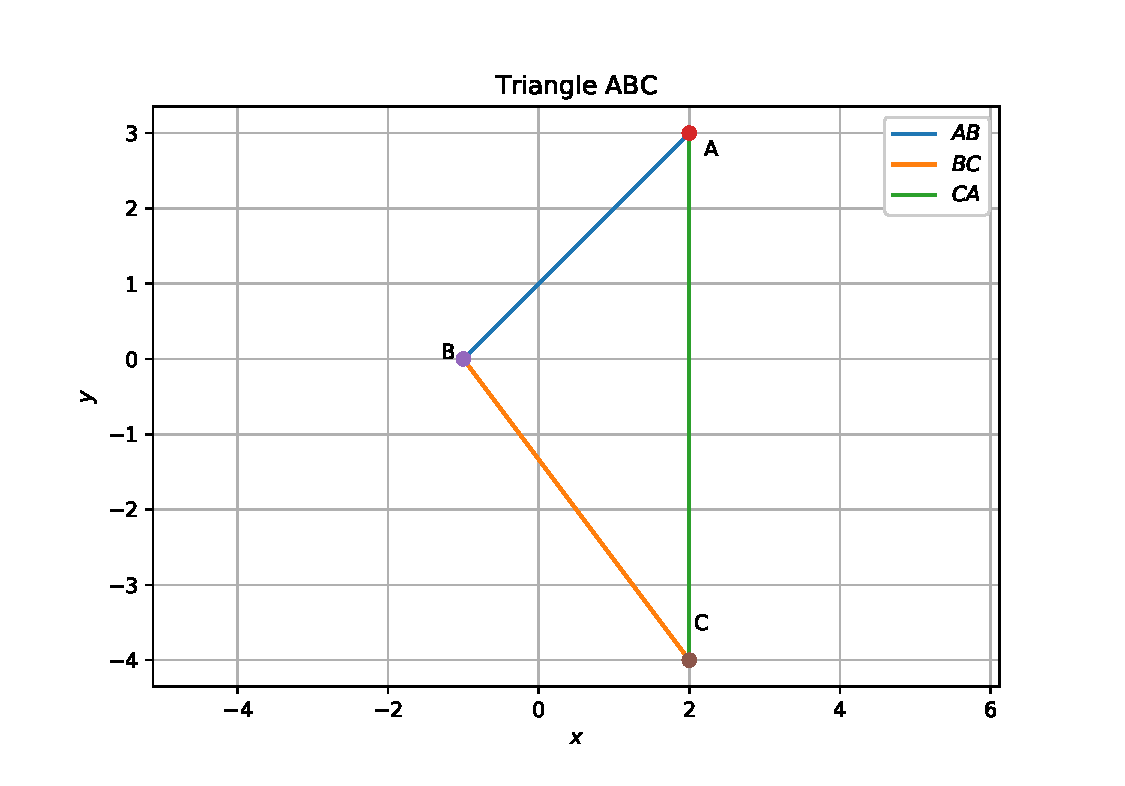
\includegraphics[width=\columnwidth]{./codes/triangle/triangle1.eps}
\caption{Triangle $ABC$ using python}
\label{fig:triangle_1}
\end{figure} 

\item The area of triangle $PQR$: \\
\solution The area of triangle $PQR$ using Heron's formula is obtained as:
$$\frac{1}{2}\norm{(\vec{Q}-\vec{P})\times(\vec{R}-\vec{P})}$$
and it is found in the following python code:
\begin{lstlisting}
codes/triangle/tri_area_PQR.py
\end{lstlisting} 

Area of $\triangle{PQR}$ = $32 units^2$
$\triangle{PQR}$ in Fig.\ref{fig:triangle_2}  is generated using the following python code
\begin{lstlisting}
codes/triangle/triangle2.py
\end{lstlisting}
\begin{figure}[!ht]
\centering
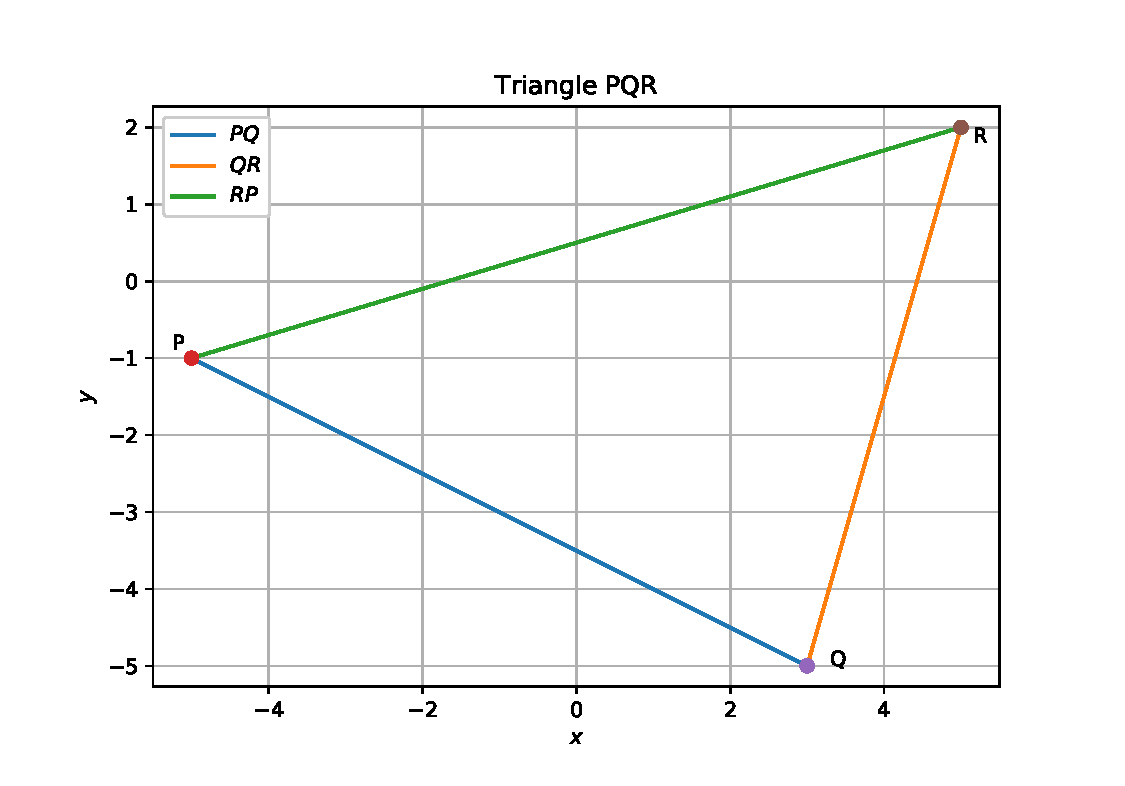
\includegraphics[width=\columnwidth]{./codes/triangle/triangle2.eps}
\caption{Triangle $PQR$ using python}
\label{fig:triangle_2}
\end{figure} 
\end{enumerate}